% The key aspects to preserve are the \chapter, the \bibliography, and the \subappendices commands. For the rest, there should be full flexibility
\chapter{Title paper 1}

%% Text of abstract
\begin{abstract}
\noindent   \lipsum[9-9]
\end{abstract}

\noindent   \textit{Keywords:}      \newline
            \textit{JEL Codes:}



\pagebreak
\setlength\epigraphwidth{10cm}
\setlength\epigraphrule{0pt}
\epigraph{      \flushright{\textit{Quote for Paper 1}} }   

% main text
\section{Introduction}

% For example, I implement this strategy... 

\lipsum[11-11] Table (\ref{paper1_summary_stat}) shows...

\begin{table}[ht]
    \centering
{
\def\sym#1{\ifmmode^{#1}\else\(^{#1}\)\fi}
\begin{tabular}{l*{1}{ccccc}}
\hline\hline
       %             &Summary Statistics&            &            &            &            \\
                    &Observations&        Mean&          SD&         Min&         Max\\
\hline
Price               &          74&    6165.257&  (2949.496)&    3291.000&   15906.000\\
Mileage             &          74&      21.297&     (5.786)&      12.000&      41.000\\
Repair              &          69&       3.406&     (0.990)&       1.000&       5.000\\
Headroom            &          74&       2.993&     (0.846)&       1.500&       5.000\\
Trunk               &          74&      13.757&     (4.277)&       5.000&      23.000\\
Weight              &          74&    3019.459&   (777.194)&    1760.000&    4840.000\\
Length              &          74&     187.932&    (22.266)&     142.000&     233.000\\
\hline\hline
\end{tabular}
}
\caption{Summary Statistics}
\label{paper1_summary_stat}
\end{table}  




\section{The analysis}

\lipsum[8-8] As in table (\ref{paper1_table_frequency}). The first mention of an acronym refers to what it means: \gls{usa} (as described in \citet{krugman2010theory}). And there is \cite{woessmann2016importance}...

\begin{center}
    \vspace{0.3cm}
    \textit{[Table \ref{paper1_table_frequency}]}
    \vspace{0.3cm}
\end{center}

\begin{figure}[hbt!]
    \centering
    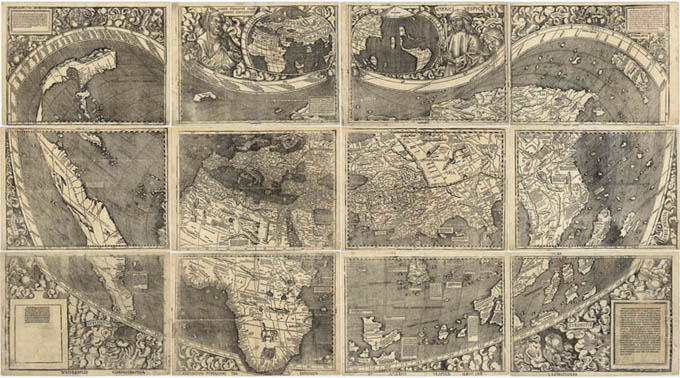
\includegraphics[width=0.9\textwidth]{graph_and_picture/Waldseemuller_map.jpg}
    \caption{A map}
    \label{chapter1_map_waldseemuller}
\end{figure}



% Bibliography Paper 1
\pagebreak
\bibliographystyle{\stylechoice}
\bibliography{Bibliographies/Paper1.bib}


% If you put main tables/maps/graph, etc. outside the main text but not in Appendix:
\pagebreak
\section*{Tables (if put in the end of the paper)}

\begin{table}[h!]
    \centering
    \begin{tabular}{cccc}
\hline \hline
\multirow{2}{*}{Frequency} &   & \multicolumn{2}{l}{Region}       \\
                           &   & A           & B                  \\
\hline                           
\multirow{2}{*}{Period}    & 1 & 78521          & 3982            \\
                           & 2 & 54246          & 3521            \\
\hline \hline
    \end{tabular}
    \caption{Frequency Table}
    \label{paper1_table_frequency}
\end{table}  



% Appendices Paper 1
\pagebreak
\begin{subappendices}

\section{The colors on the maps}
\lipsum[10-10]

\section{{The origin of the map}}
\lipsum[11-11]


\end{subappendices}